\chapter{Review of multi- and many-core processing models}
\section{Multicore CPU architectures}
\section{Many core GPU architectures}
\subsection{Historical development}
Today's modern programmable GPU devices have evolved from the fixed-pipeline graphics hardware of the 1980's and 1990's. Driven by the demand
for high resolution graphics in the video game industry modern devices must be able to render billions of pixels per second (72 giga pixels per second 
for the latest Maxwell GTX980 devices \cite{gtx980}). As such these devices are geared towards achieving high throughput over higher operational latencies compared to traditional
CPU-based computing. The steps involved with transforming primatives (typically triangles) in world space to rasterized images rendered by a display takes thousands
of compute cycles from start to finish. However the coordinate, lighting and per-pixel shading operations are highly data-parallel operations. In addition the stages within
the graphics pipeline can be computed in parallel; while new primatives enter the pipeline the rasterization and fragment processing of primatives previously transformed is 
completed, enabling both data- and task-parallelism on GPUs. The major steps in the graphics pipeline is shown in Figure~\ref{fig_graphics_pipeline} for reference.

\begin{figure}[ht!]
 \begin{mdframed}
 \centering
  \begin{tikzpicture}[node distance=2.8cm,  
    block/.style={
      draw,
      fill=white,
      rectangle, 
      text width=2.0cm,
      inner sep=0.2cm}]
    \node (app) [block] {3D application / game};
    \node (api) [block, right of=app] {3D API \& drivers};
    \node (fe) [block, below of=app] {GPU front end};
    \node (assembly) [block, right of=fe] {Primitive assembly};
    \node (rasterization) [block, right of=assembly] {Rasterization and interpolation};
    \node (rasterops) [block, right of=rasterization] {Raster operations};
    \node (fb) [block, right of=rasterops] {Framebuffer};
    \draw [dashed,transform canvas={yshift=-1.4cm}] ($(app) - (0.5cm,0)$) -- (fb |- app) node [right, above] (cpu) {CPU} node [right, below] (gpu) {GPU};
    \draw [rarrow] (app) -- (api);
    \draw [rarrow] (api) -- (fe);
    \draw [rarrow] (fe) -- (assembly);
    \draw [rarrow] (assembly) -- (rasterization);
    \draw [rarrow] (rasterization) -- (rasterops);
    \draw [rarrow] (rasterops) -- (fb);
  \end{tikzpicture}
 \caption[Graphics pipeline]{The classical graphics pipeline. At the front end of the pipeline verticies are transformed, colours assigned,
 texture coordinates and normals calculated. The rasterization step interpolate per-vertex data, such as colour accross all the pixels 
 touched by the triangle formed between vertex tripples. Raster operations performs final blending and anti-aliasing operations, before the images written
 out to the display frame buffer.}
 \label{fig_graphics_pipeline}
 \end{mdframed}
\end{figure}

The requirement of transforming, rasterizing and shading possibly millions of triangle primatives driving GPU development clearly diverges from the requirements behind the
design of traditional CPUs. CPU development is driven by the need to process large sequential programs per CPU core, each containing complex branching and diverse memory access patterns, 
whereas GPUs are driven by the need to apply the same set of basic operations to many elements (or ``Single Instruction Multiple Data'' [SIMD]) paradigm that graphics processing subscribes to. 
Whereas CPUs use several tiers of large caches to hide the latencies of memory accesses GPUs have relatively little on-chip cache memory per basic compute (``Streaming Processor'' [SP]) 
unit. Instead of caching GPUs rely mostly on the amount of parallel work available to each SP unit and a fast context switching / work scheduling mechanism to ensure each of the SPs are 
occupied with work while memory transactions are completed for threads stalled by load and store operations.

Although the hardware platform could potentially be employed for applications other than 3D graphics it wasn't until the early 2000's that programmable graphics hardware became widely
available. For instance the NVIDIA GeForce 3 exposed the internal instruction set of the vertex processor to the application developer. Soon the ATI Radion 9700 and GeForce FX 
made the fragment shading process normally part of the rasterization and interpolation step reprogrammable. At this point the vertex and fragment shading units were run on seperate
hardware. The XBox 360 (2005) introduced an early unified vertex and fragment shader processor.

Even though the hardware now supported extending the traditional graphics pipeline to do more complex operations it was still impractical to use the highly parallel hardware for 
computational processes other than graphics on any large scale products. Computational problems had to be mapped to the standard graphics operands: verticies and textures. Other problems
such as the lack of scattered memory writes limited the applicability of the platform to a small number of problems.

This was addressed by a series of software (along with necessary hardware modifications) developments that aimed to to give application developers access to the processors without having to call
on Graphics APIs. Of those developments BrookGPU \cite{buck2004brook} was an early abstraction away from graphics primatives. It recasted computation in terms of small programs (``kernels'') operating
on ``streams'' of input data elements (arrays of values that can be operated on in parallel). This paradigm sets GPUs aside from ordinary vector processors that loads a series of values from global
memory, performs a simple mathematical operation on each of the elements and write the results back to global memory. Instead stream processors can load values from local register memory, performing multiple
operations on each of these values before storing the results (possibly to local memory). The paradigm allows for achieving greater arithmetic intensity (a single memory operation is followed
by many computations) and is critical for hiding the high latencies of memory accesses experienced on GPUs. 

More recently NVIDIA's CUDA \cite{cuda} and the OpenCL \cite{opencl} have become the defacto standard ways of 
programming GPUs to perform general scientific computing used in a variety of fields including the signal 
processing domain. Both lend themselves to the streaming processor paradigm and facilitate the implementation
of the following generally-used parallel computing primatives:
\begin{itemize}
 \item Scatter/gather: The addresses used in memory accesses (both load and store) can be computed.
 \item Map: an operation is applied to every element in the stream. Typically many threads will be launched
       each reading an element from the stream, performing the operation on that element and writing the value
       back to memory afterwards.
 \item Reduce: By applying a binary associative operation repeatedly a sequence of values is reduced to a single value.
       An example is ordinary summation, minimums/maximums, variance, etc. These operations typically split the data up into
       subsets, performing many additions in parallel and repeating the process on the set of results until a single value is
       obtained. 
 \item Scans: Scan and prefix scan operations are widely used in parallel programming (for instance index calculations as used
       in our work). A scan of an array contains the running accumulations (in the case of summation) of elements in an array. 
\end{itemize}

\subsection{Modern programmable GPU architecture}
The difference in design philosophy is reflected in the substantial differences in the architectures of modern GPUs and CPUs. CPUs dedicate a significant portion die area to large caches and complex control logic dealing with
branch prediction and scheduling. GPUs on the other hand dedicate a significant portion of die area to arithmetic and other execution units and rely on having enough arithmetic work to occupy most of those units most of the time.
Figure~\ref{fig_cpu_gpu_diff} illustrates the proportions of both CPU and GPU die area spent on artithmetic.
\begin{figure}[ht!]
 \begin{mdframed}
  \centering
  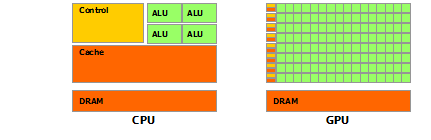
\includegraphics[width=0.5\textwidth]{images/gpu-devotes-more-transistors-to-data-processing.png}
  \caption[CPU vs. GPU architecture]{The proportion of transistors allocated to arithmetic processing in CPUs and GPUs. Taken from the NVIDIA programming reference \cite{cuda}}
  \label{fig_cpu_gpu_diff}
 \end{mdframed}
\end{figure}

Modern GPUs works best in problem contexts where a significant portion of the computation is data-parallel. In CUDA nomenclature (similar concepts exist in OpenCL) the parallel work is broken up into a \textit{grid} of
separate thread \textit{blocks} (see Figure~\ref{fig_grid_blocks} for an illustration). In each of these blocks on-chip memory resources is shared, limiting the size of the individual blocks. On current NVIDIA GPUs there is a hard limit (1024) to the number of threads size, 
however the amount of special memory (including register memory) available to each of these blocks may further limit the number threads in the block that can physically execute simulaniously. Each of the 
blocks would therefore process a portion of stream memory. Blocks are in turn subdevided into \textit{warps} of threads (currently 32 threads form a warp) that execute instructions in lockstep. This means that when one
thread inside a warp is stalled (for instance a memory access or a synchronization barrier) the entire warp is stalled. Unlike the instruction scheduling units of CPUs the schedulers in GPUs also don't contain complex branch prediction logic; when some
threads in a warp require the execution of one of the directions in a branch while the rest take another direction both sides of the branch is evaluated and the results are simply masked out for the threads that are uneffected
by the branch. This places a heafty penalty on branch divergence within the instruction kernels and memory accesses that don't adhere to the alignment specifications of the GPU. Note that this description of how work is layed out in a high level programming language is independent of specifics of the device the work is to be run on. The individual blocks can be mapped onto the targeted device
in any order and in any quantity, depending on the resources of the device. Each block of work should therefore perform its computation in isolation of the remaining blocks. Although intra-block communication between threads 
and synchronization is possible, inter-block communication is only possible through accesses to off-chip memory and should be avoided.
\begin{figure}[ht!]
 \begin{mdframed}
  \centering
  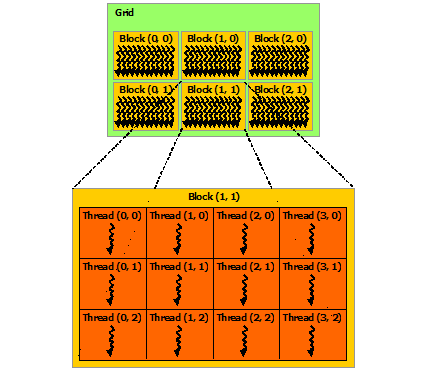
\includegraphics[width=0.3\textwidth]{images/grid-of-thread-blocks.png}
  \caption[Thread layout in CUDA]{The layout of work threads in CUDA. Taken from the NVIDIA programming reference \cite{cuda}}
  \label{fig_cpu_gpu_diff}
 \end{mdframed}
\end{figure}

At a hardware level GPUs comprise of multiple \textit{Streaming Multiprocessors}, each containing many \textit{Stream Processors} capable of performing arithmetic (predominantly IEEE 754 single precisision floating point) along
with several special function units, warp-schedulers and memory load/store units. Figure~\ref{fig_kepler_arch} shows the layout of Kepler-generation NVIDIA GPUs. The exact number of Streaming Multiprocessors and Stream Processors
vary between generations of GPUs, but the total number of Streaming Multiprocessors per GPU tend to double every 2 years. Depending on resource constraints of each of the thread blocks several blocks may be mapped to a single 
Streaming Multiprocessor for simultanious execution. The warp schedulers schedule warps that have instructions (along with the required operand data) ready for execution onto sets of Stream Processors, dispatching independent 
instructions onto individual Stream Processors per clock cycle (depending on the number of dispatch units available per Multiprocessor). Warps that are stalled (for example waiting on a load/store operation) is switched out of context
and replaced with warps that have operands ready for processing, thereby hiding memory access latencies. Ideal kernels should therefore:
\begin{itemize}
 \item Contain enough independent arithmetic instructions to occupy all the Stream Processors during
       any given clock cycle.
 \item Access to both on- and especially off-chip memory should be kept to a minimum and subscribe to coalesced access patterns, especially considering that the number of load/store units are far fewer than the number of
       single precision units and peak memory bandwidth is on the order of 60x lower (Kepler generation) than peak single precision compute throughput of the device. In other words the arithmetic intensity should be high, as
       is the case in typical graphics shading operations for instance.
 \item There must be enough warps of work scheduled to the GPU to keep the Multiprocessors occupied most of the time.
 \item Special memory resources (including registers) should be used sparingly to ensure the Streaming Multiprocessor is not starved of resources as this lowers the number of warps that can be executed at any given point in time 
      (``effective occupancy'').
\end{itemize}
\begin{figure}[ht!]
 \begin{mdframed}
  \centering
  \begin{subfigure}[b]{0.7\textwidth}
    \centering
    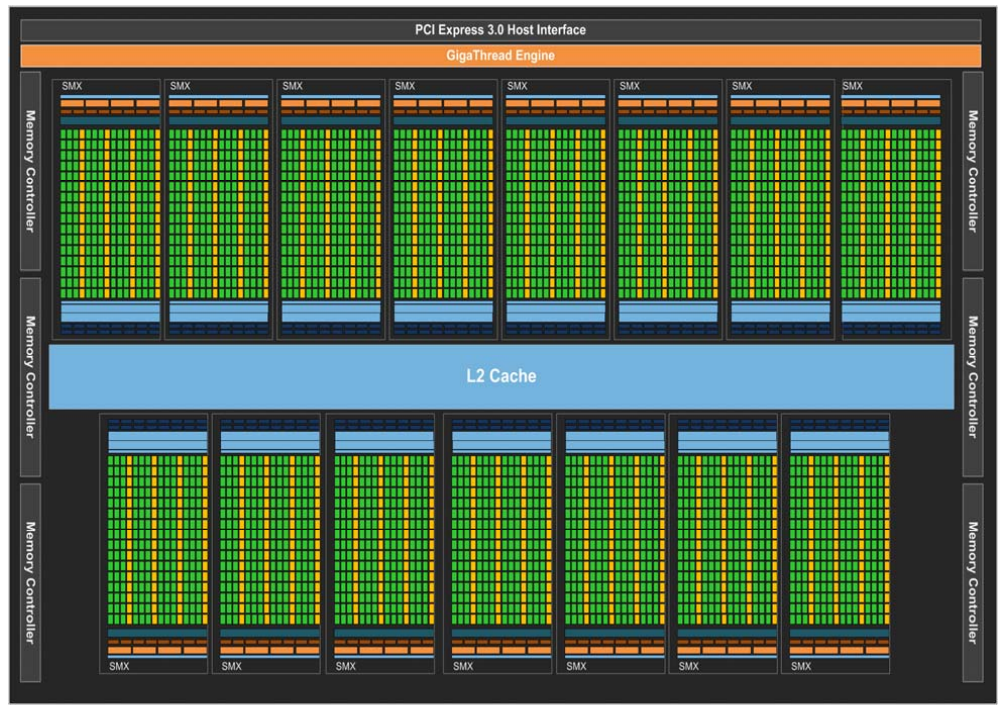
\includegraphics[width=\textwidth]{images/kepler_arch.png}
    \caption{}
  \end{subfigure}
  \begin{subfigure}[b]{0.6\textwidth}
    \centering
    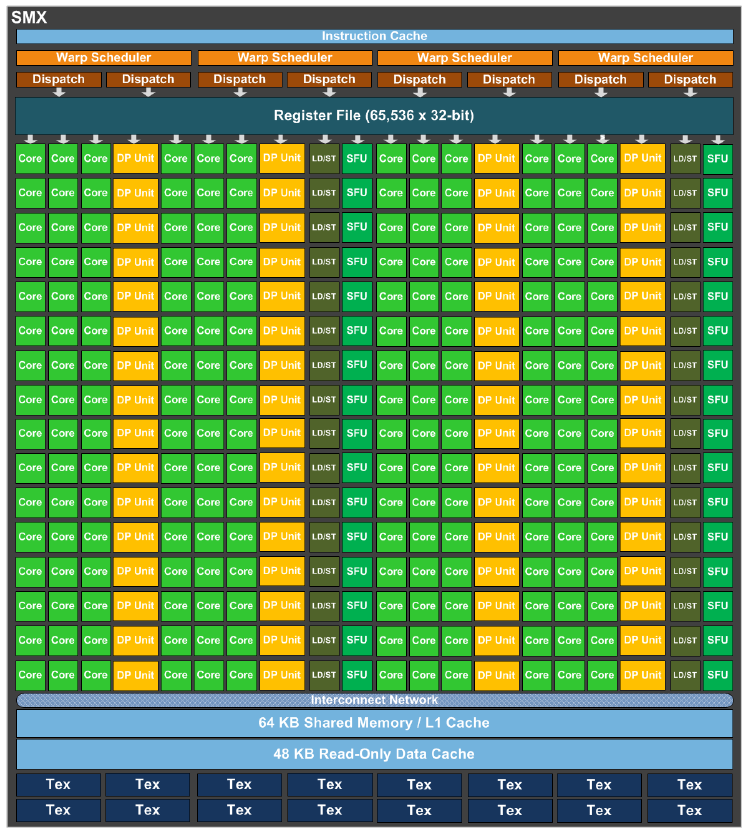
\includegraphics[width=\textwidth]{images/kepler_smx_arch.png}
    \caption{}
  \end{subfigure}
  \caption[Kepler architecture]{Kepler die architecture. (a) shows the overall die layout, containing 15 Streaming Multiprocessors. (b) shows the layout of each multiprocessor, containing one double precision unit for every 
				3 single precision units, 1 load/store and 1 special function unit for every 6 single precision units. The total number of registers, local and shared memory is split between the number of threads per 
				block, determining how many blocks can be executed simultaniously. Taken from the Kepler whitepaper \cite{kepler}}
  \label{fig_kepler_arch}
 \end{mdframed}
\end{figure}
\subsection{GPU memory layout}